%%%% Proceedings format for most of ACM conferences (with the exceptions listed below) and all ICPS volumes.
\documentclass[sigconf]{acmart}
%%%% As of March 2017, [siggraph] is no longer used. Please use sigconf (above) for SIGGRAPH conferences.

%%%% Proceedings format for SIGPLAN conferences 
% \documentclass[sigplan, anonymous, review]{acmart}

%%%% Proceedings format for SIGCHI conferences
% \documentclass[sigchi, review]{acmart}

%%%% To use the SIGCHI extended abstract template, please visit
% https://www.overleaf.com/read/zzzfqvkmrfzn


\usepackage{booktabs} % For formal tables

% Copyright
\setcopyright{none}
%\setcopyright{acmcopyright}
%\setcopyright{acmlicensed}
%\setcopyright{rightsretained}
%\setcopyright{usgov}
%\setcopyright{usgovmixed}
%\setcopyright{cagov}
%\setcopyright{cagovmixed}


% DOI

% ISBN

%Conference
%\acmConference[WOODSTOCK'97]{ACM Woodstock conference}{July 1997}{El
%  Paso, Texas USA} 
%\acmYear{1997}
%\copyrightyear{2017}


%\acmArticle{4}
%\acmPrice{15.00}

% These commands are optional
%\acmBooktitle{Transactions of the ACM Woodstock conference}
%\editor{Jennifer B. Sartor}
%\editor{Theo D'Hondt}
%\editor{Wolfgang De Meuter}


\begin{document}
\title{Predictive flood alerts through crowdsourced data}

\author{Abraham Quintero}
\affiliation{%
  \institution{Massachusetts Institute of Technology}
}
\email{abrahamq@mit.edu}

\begin{abstract}
The Riskmap System allows users to report flooding through social media. 
It also allows Emergency Operations Centers (EOCs) to communicate 
with users through a public map interface where EOC managers can 
highlight dangers. Here we present a novel system for helping 
disaster personnel identify the most relevant social media reports of flooding.
\end{abstract}

%
% The code below should be generated by the tool at
% http://dl.acm.org/ccs.cfm
% Please copy and paste the code instead of the example below. 
%
\begin{CCSXML}
<ccs2012>
<concept>
<concept_id>10002951.10003227.10003241.10003243</concept_id>
<concept_desc>Information systems~Expert systems</concept_desc>
<concept_significance>300</concept_significance>
</concept>
</ccs2012>
\end{CCSXML}

\ccsdesc[300]{Information systems~Expert systems}

\maketitle

\section{Introduction}
South and South East Asian countries are among the most vulnerable regions. Sea level rise and climate change induced extreme weather events promise to create even more damage related to natural disasters.Every monsoon season, coastal mega-cities like Jakarta, Mumbai, Chennai, Dhaka routinely experience extreme rainfall events that results in sever flooding.  ; however, 
by utilizing citizens as sensors, the Riskmap system 
has been able to produce highly accurate flood maps that 
reduce government response to disaster events and also help 
future planning. 

One problem that still remains is that of information overload. 
Each citizen report contains an estimated flood height, a gps coordinate, 
a picture, and a textual description. During disaster events, thousands 
of reports are input into the system, thus creating information overload 
for the disaster managers that are tasked with manually reviewing them.

% TODO: This is bad writing
Here we use a combination of pre-trained  machine learning tools 
combined using simple methods to classify whether an incoming report belongs 
to a 'High Flooding' event. Furthermore, this system is able to explain its decisions 
by showing emergency managers which specific features of the report were most important in its choice.

\begin{figure}[ht]
    %%TODO: ask adi for system diagram 
    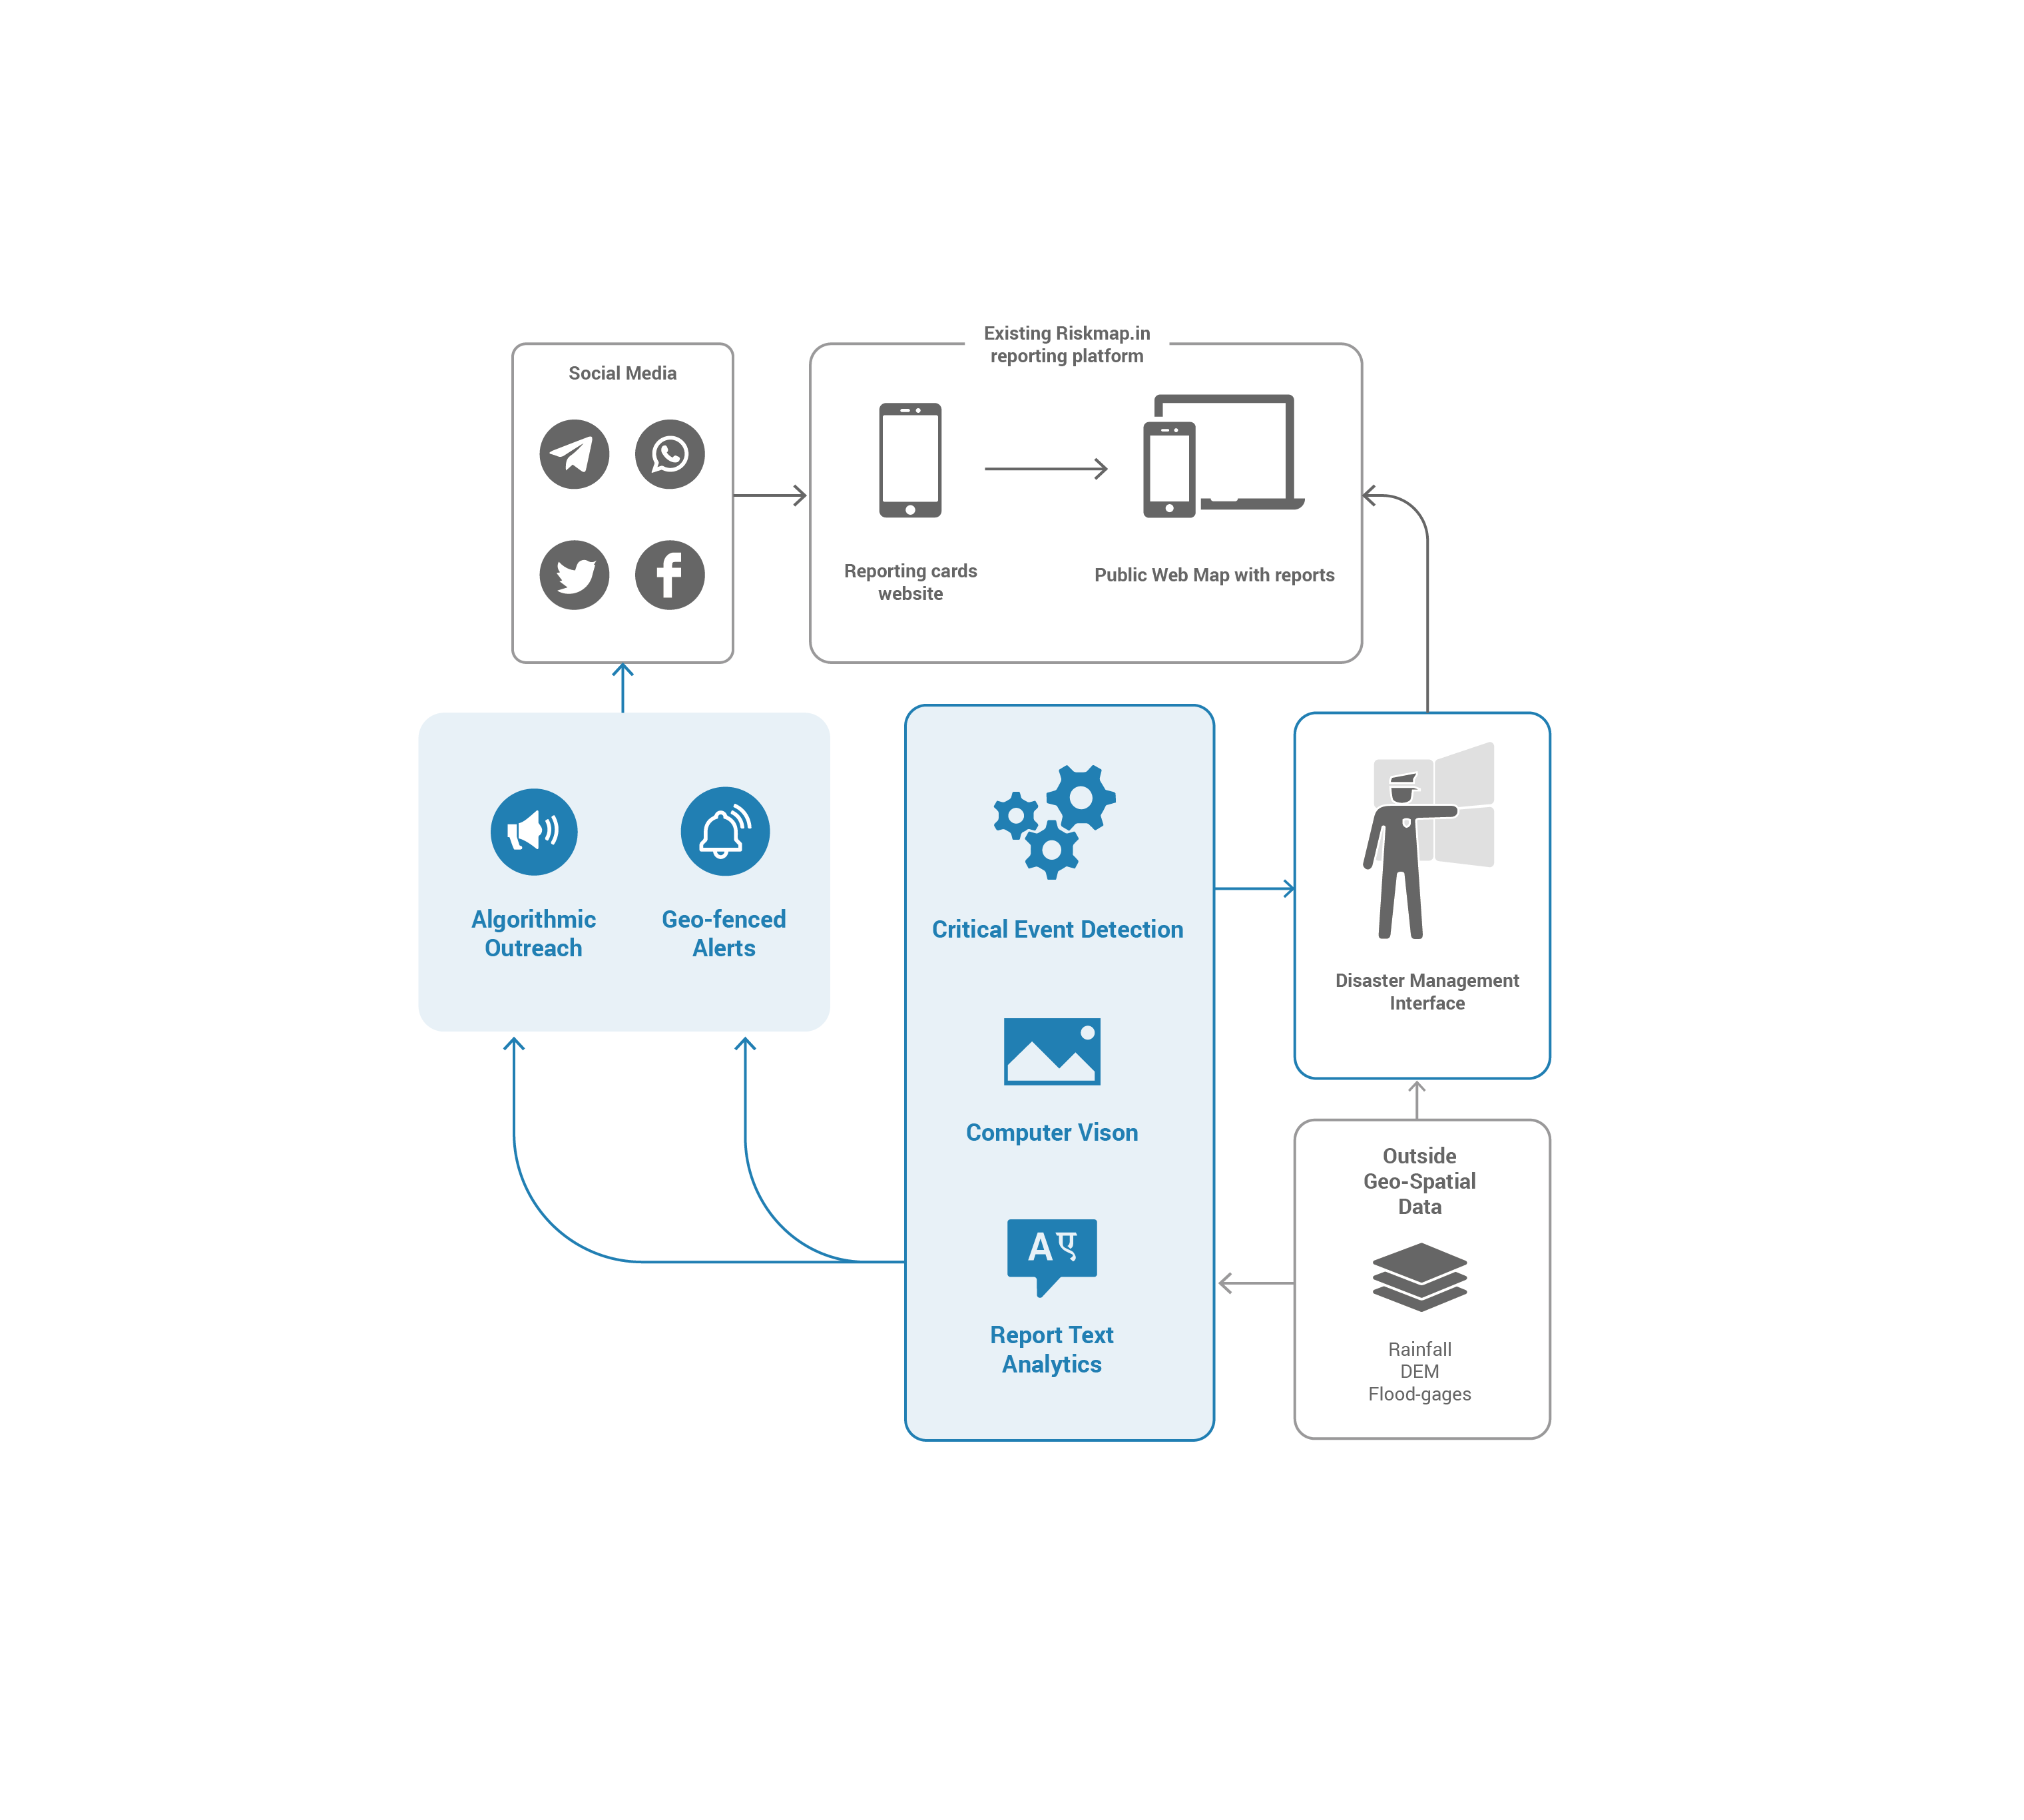
\includegraphics[width= 95mm]{high_level.png}
    \caption{Riskmap System Diagram}
\end{figure}

\begin{figure}[ht]
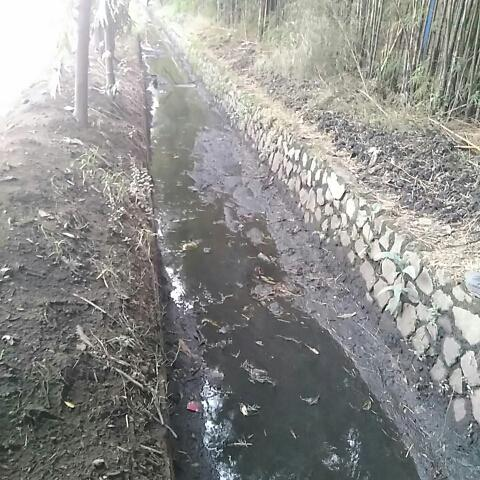
\includegraphics[width = 85mm]{clogged_drain.jpeg}
\caption{Example of a clogged drain report image}
\label{fig:clogged_drain}
\end{figure}

\section{Datasets}
The Riskmap project has collected over 5000 reports from Jakarta through a 
variety of social media reporting streams. These include Twitter, Facebook, and 
Qlue (an app provided by the government of Jakarta) among others. In this corpus, 
there are 4900 images and 5200 textual descriptions in Indonesian. Of those reports, 
1129 have been labeled by the government of Jakarta as being heavy flooding.

In Chennai, the Riskmap project has recorded over 300 images and 430 textual descriptions. 
The reports have been labeled with the help of a partner organization on the ground.

\section{Challenges}
Whether there is heavy flooding is a highly localized and subjective decision. It is 
not a simple binary classification as we have modeled it for this project. In 
order to deal with the noisiness of the labeling, an ensemble learning approach 
will be used\cite{ensemble}. Ensemble learning will help us to use many weak 
predictors in order to create a single strong indicator of the probability that 
a report signifies heavy flooding.

\section{Utilizing user provided image data}
\subsection{Introduction}
Image data provides an incredible resource for information extraction in disaster 
scenarios \cite{}



The first challenge is understanding how to utilize image data. One simple method would be to use 
a pre-trained multilabel classifier that includes 'Flood' as one of its labels. 

AWS Rekognition provides one such pre-trained classifier through its \textbf{detect\_labels} api. Classifying all the pictures in the Jakarta dataset (4900 images) 
reveals that 1600 of them have 
a 'Flood' label that has a confidence score of greater than .5. 

On the surface that seems promising, but plotting the results shows that using only 
this one feature creates a dataset that is not linearly separable. Adding more 
labels from the image classification, thus increasing the size of the feature space, 
will help us to differentiate between images that depict heavy flooding and those that 
are pointing out light flooding or clogged drains such as \ref{fig:clogged_drain}.

Perhaps we can choose labels that we think might be important- for example, 
maybe heavy flooding means that there won't be vehicles on the road so we can 
add the 'Vehicle' label. Or maybe we think that there might be 'Cars' but not 'Motorcycles' 
during heavy flooding. 

How do we go about choosing which labels are best?
If we train a classifier on the entirety of the data, and then see which classes have 
the most weight on the separator then we can find which labels are the most useful in 
separating flooding from non flooding images. 
\\
Carrying out this process using the perceptron algorithm shows that the 10 most important classes are: 

['Planter', 'Slum', 'Strap', 'Sedan', 'Grove', 'Parade', 'Ground', 'Vacation', 'Coupe', 'Trail']

\subsection{Evaluation}
The separator created by perceptron has an average .80 percent test success rate at classifying heavy 
flooding images from both datasets. 

\begin{figure}[ht]
    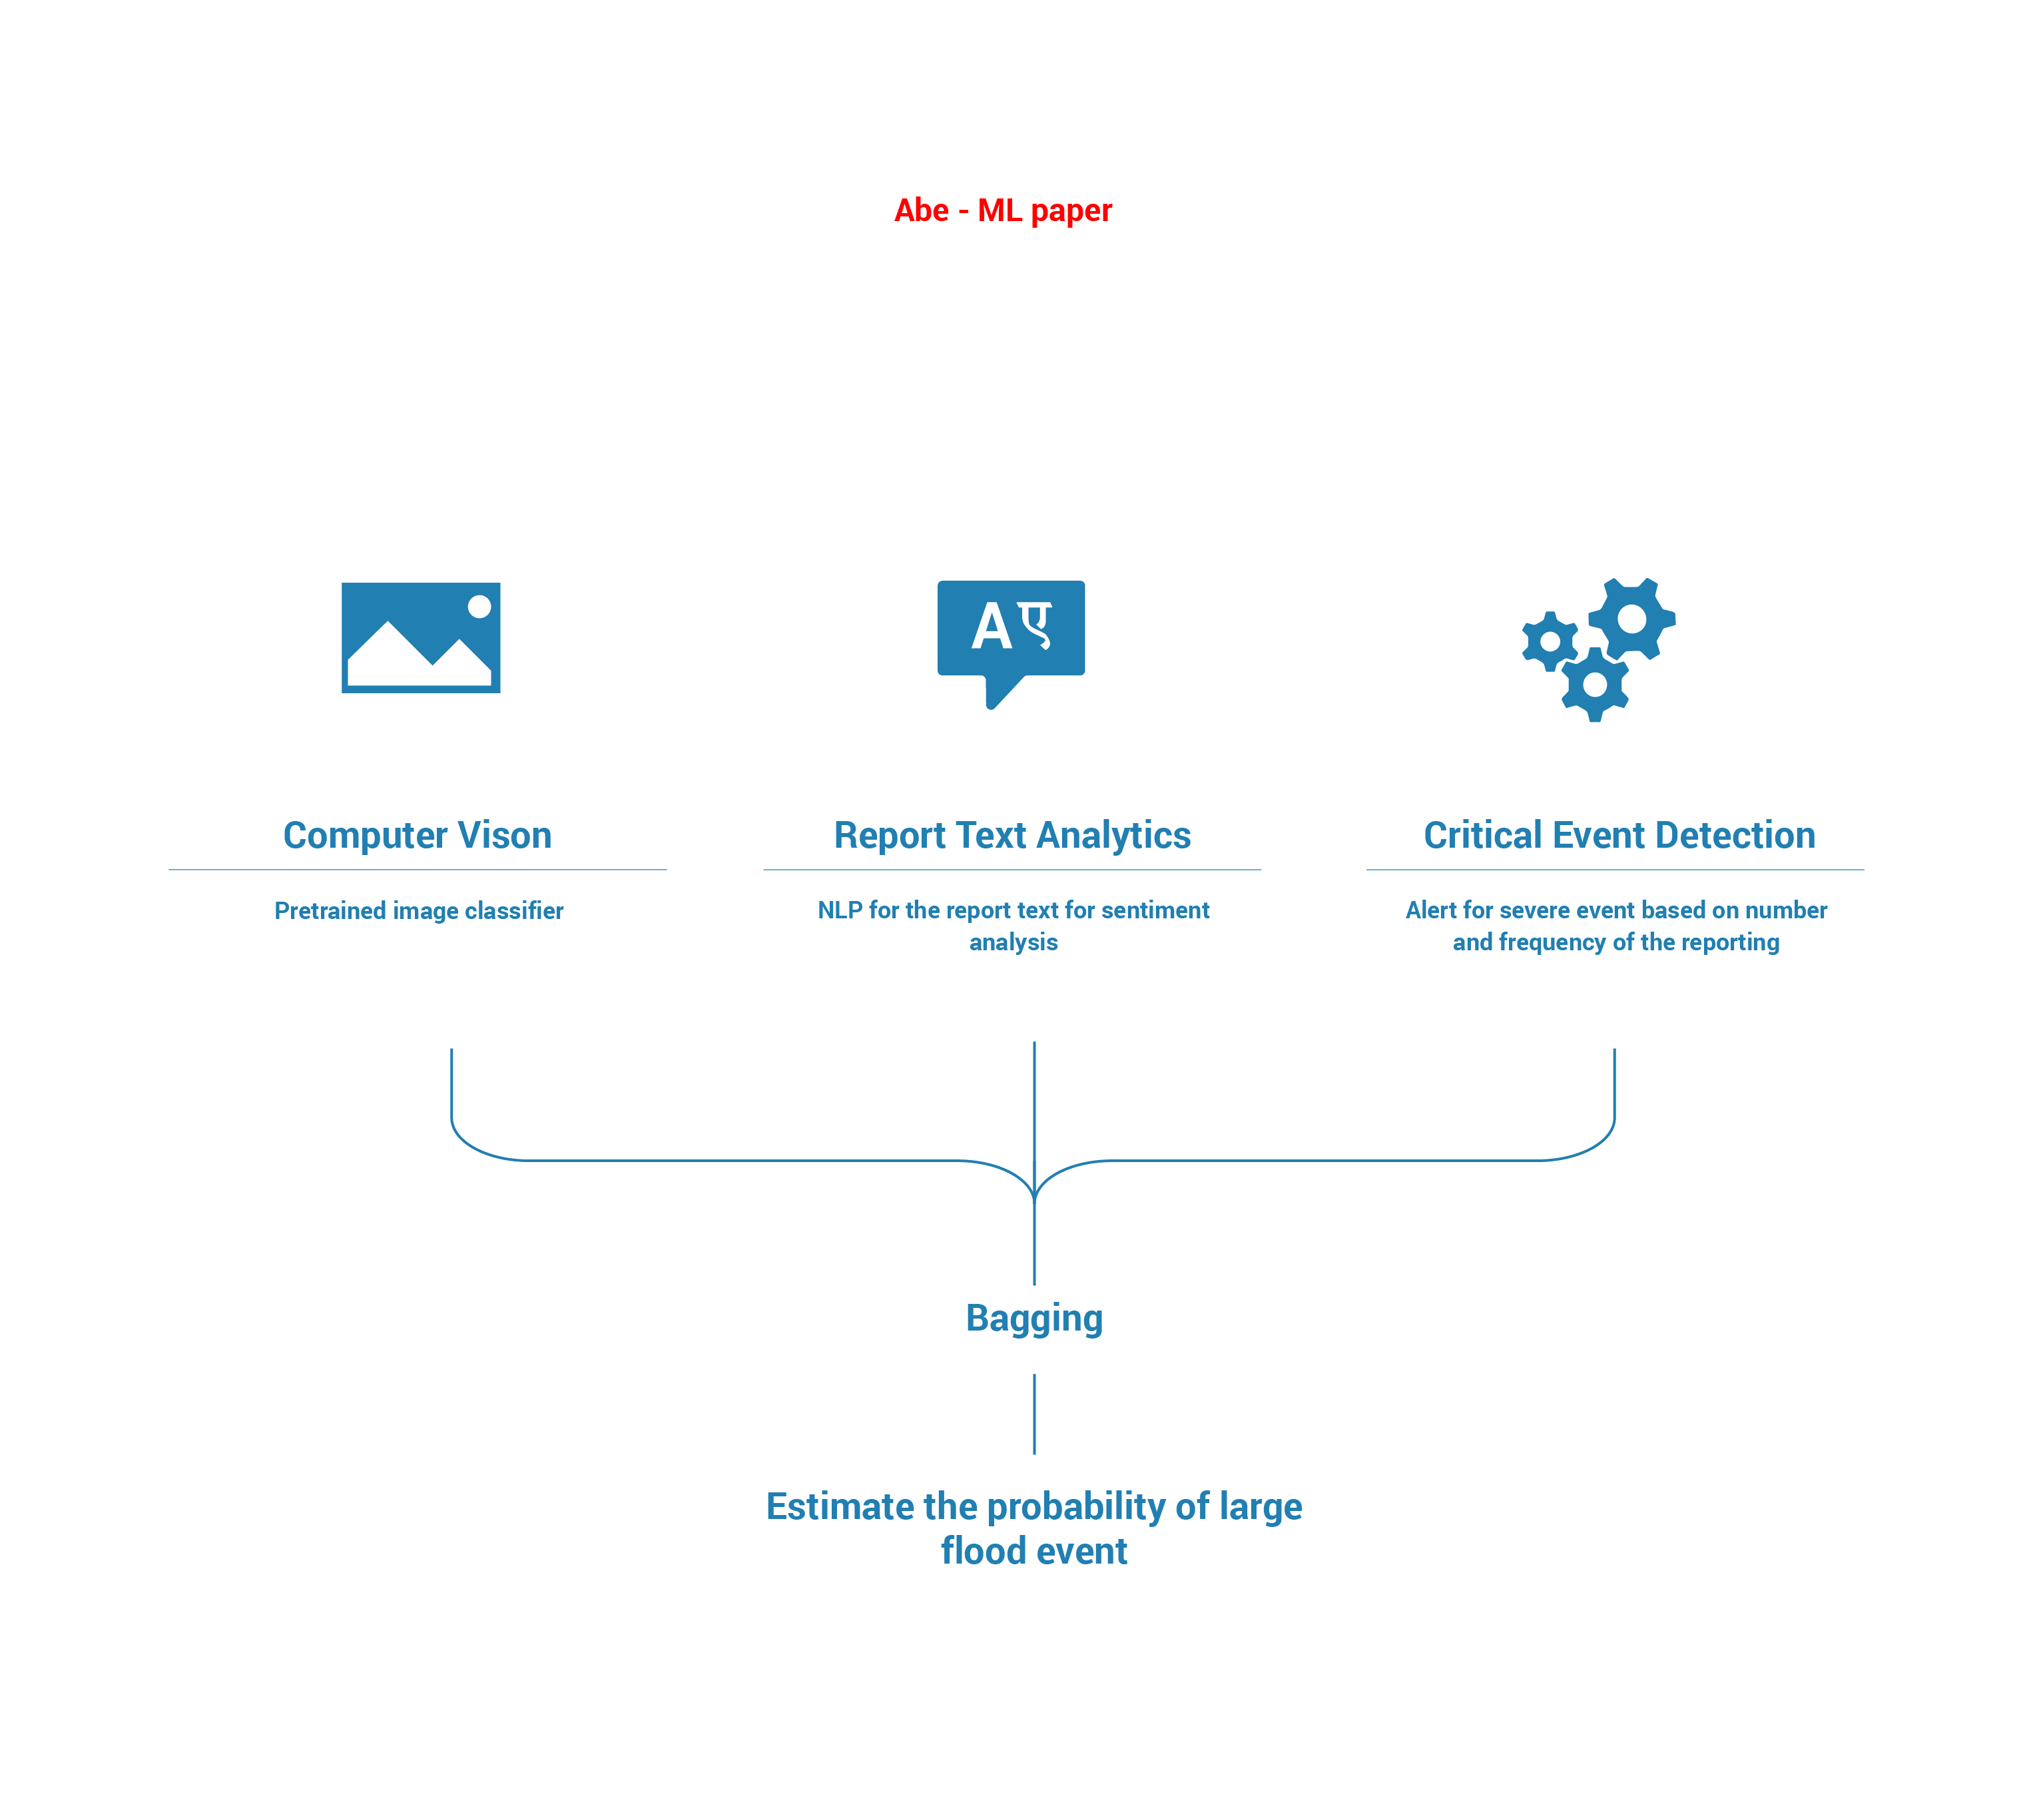
\includegraphics[width = 85mm]{ml_diagram.png}
    \caption{bagging}
    \label{fig:bagging}
\end{figure}


\section{Sentiment analysis on textual descriptions}
Since each report in the Chennai dataset includes a textual description in English, 
we can use off the shelf sentiment analysis to gauge how
negatively citizens are feeling. We can investigate the relation between a negative sentiment and 
heavy flooding by using conditional probability. Let's say that a text is mainly negative if 
its negative sentiment is greater than half, then the true positive rate is given by 
\\
$$P( Heavy Flooding | negative) =  \frac{P(heavy Flooding | negative)}{P(negative)} = .65 $$
\\
while the false positive rate is given by
\\
$$P( No Flooding | negative) =  \frac{P(No Flooding | negative)}{P(negative)} = .34 $$
\\

This statistic shows that while there is some relation between a negative sentiment and flooding, it is not 
a very strong signal. Again, trying to separate the data using just this method is impossible.

\section{Estimated Flood height}
The simplest data to interpret is the estimated flood height that users input into a flood report. 
On the surface, this provides an easy way to separate the data- if users estimate a high flood then 
this is high flooding, right? However, the data has incredible amounts of noise because a 
large amount of users 
did not change the \textbf{flood\_height} parameter when they were inputting their reports. As 
a result of this, over 10 percent of heavy flood reports were submitted with the default flood height, 50 cm.

\section{Moving Average Thresh Holding}
The number of reports that are coming into the system also 
provide a signal into the urgency of the flood
event. During times of heavy flooding the 
number of reports per hour increases. Taking a moving average and 
thresh holding to create a binary signal allows us to get a 
rough signal of times that an above average 
number or reports are coming into the system. 
Figure \ref{fig:moving_avg} shows the count of reports binned
by the hour, while the red line shows the moving average with a thresh hold of 5.

\begin{figure}[ht]
    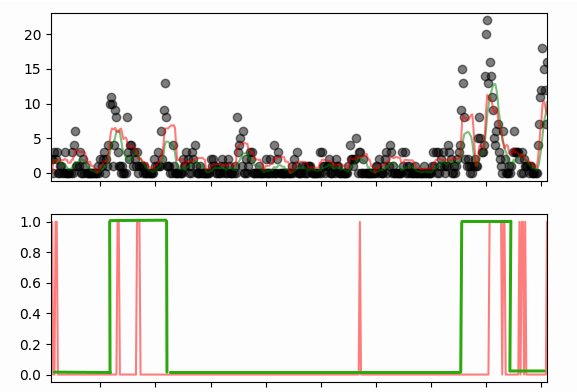
\includegraphics[width = 85mm]{moving_avg_jakarta.png}
    \caption{Number of reports binned by hour, red line shows the moving average signal signal while 
    green is ground truth known heavy flooding}
    \label{fig:moving_avg}
\end{figure}

\section{Implementation}
The pre-trained image classification was accomplished 
using the AWS Rekognition API with the boto3 library 
\cite{boto}.

Using the AWS api means that whenever the AWS model 
gets better our system will also benefit from that
increase in performance. Furthermore, it means
that we do not have to incur the costs of training a
general image classifier.

The input feature vector for the 
bagging network was created using python, the AWS boto3 library, and numpy.

This vector composes the output of the machine learning algorithms described
above
\\

\begin{align}
    X = \begin{bmatrix}
           signed\_dist\_from\_image\_separator \\
           negative\_sentiment \\
           flood\_height \\
         \end{bmatrix}
\end{align}

The bagging network itself was constructed using torch with three linear input
units and 1 hidden unit with ReLU activation functions, and two output units 
using log softmax to classify outputs either into the 'heavy\_flooding' or 
'no\_heavy\_flooding' category.

\section{Conclusion / Lessons Learned}
Using 5 fold cross validation, the average accuracy of the bagging network 
is .95 using the Chennai dataset and .93 using the Indonesia dataset.

\subsection{Future work}
Incorporating the temporal nature of reports into the bagging ensemble 
learner is a difficult problem. One possibility is to use a 1 dimensional 
convolution layer in order to find the temporal relationships between the data,
but interpreting such results when run through the dense bagging network is 
difficult. Instead, we have decided to output the result of streaming peak finding 
directly since the event graph is easy to interpret and provides instant 
insight into the event.

Furthermore, it may be helpful to weigh the reports by the probability that 
the bagging network believes they include heavy flooding and then use this data
as for the streaming peak finding.

Another idea for future work would be to use transfer learning in order 
to use both Chennai and Jakarta data together while predicting new reports.

\begin{thebibliography}{}
     \bibitem{ensemble}
     Training deep neural networks on noisy labels with bootstrapping
     \emph{https://arxiv.org/abs/1412.6596}
     
     \bibitem{boto}
     AWS Documentation \\
     \emph{https://boto3.amazonaws.com/v1/documentation/api/latest/reference/services/rekognition.html}

\end{thebibliography}

\end{document}